
\begin{itemize}
	\item Grafique en una sola figura la respuesta al impulso del sistema de tiempo continuo, y las dos aproximaciones
	de tiempo discreto.
\end{itemize}

Para esto se generaron dos gráficas: una sin diferenciador discreto y una con diferenciador discreto, siendo representadas por las curvas roja y amarilla respectivamente. Cabe mencionar que las curvas son la respuesta al impulso.

\noindent \textbf{Salida con $T_s=1$}

\begin{figure}[H]
	\centering
	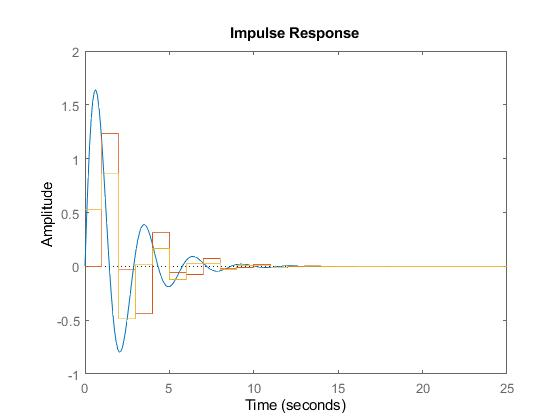
\includegraphics[width=0.7\linewidth]{SalidaTs1DosHz}
	\caption{{Salida con $T_s=1$}}
	\label{fig:salidaTs01-1}
\end{figure}



La obtención de la gráfica anterior se realizó con la siguiente serie de comandos

\begin{itemize}
\item Ts=1
\item Hs=tf([5],[1 1 5])
\item Hz=c2d(Hs,Ts)
\item Hz2=c2d(Hs,Ts,'foh')
\item impulse(Hs)
\item hold on
\item dimpulse(Hz,Ts)
\item hold on
\item dimpulse(Hz2,Ts)
\end{itemize}

\begin{itemize}
	\item Disminuya el tiempo de muestreo hasta obtener una aproximación adecuada de la respuesta del sistema
	y grafique la comparación. ¿Qué aproximación resultó mejor?
\end{itemize}

Para obtener una aproximación adecuada se disminuyó el valor de $T_s$ a 0.0001, generando la siguiente 
\newline

\noindent \textbf{Salida con $T_s=0.0001$}

\begin{figure}[H]
	\centering
	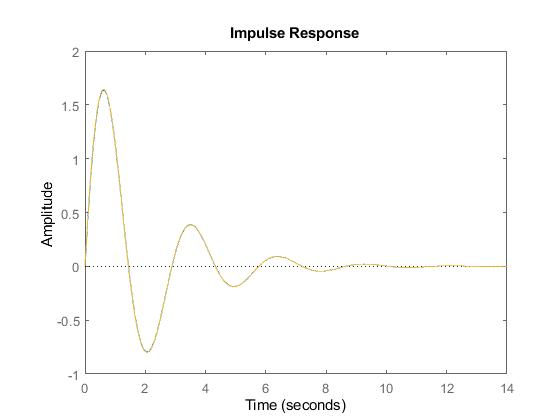
\includegraphics[width=0.7\linewidth]{SalidaTs00001DosHz}
	\caption{{Salida con $T_s=0.0001$}}
	\label{fig:salidaTs001-1}
\end{figure}

Debido a la gran aproximación de ambas gráficas se requiere de un acercamiento para poder observar las diferencias entre la gráfica generada con diferenciador (amarilla) y la generada sin diferenciador (roja).

\begin{figure}[H]
	\centering
	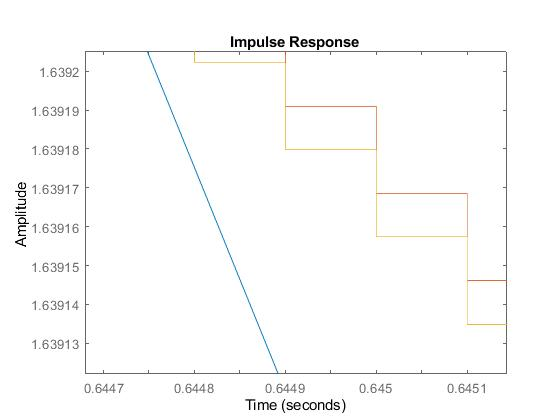
\includegraphics[width=0.7\linewidth]{SalidaTs00001DosHzAcercamiento}
	\caption{{Salida con $T_s=0.0001$}}
	\label{fig:salidaTs001-2}
\end{figure}

Gracias a este acercamiento podemos apreciar que la gráfica que se acerca más a la de tiempo continuo (azul) es la que utiliza un diferenciador (amarilla). Para esto utilizamos los comandos:

\begin{itemize}
\item Ts=0.0001
\item Hs=tf([5],[1 1 5])
\item Hz=c2d(Hs,Ts)
\item Hz2=c2d(Hs,Ts,'foh')
\item impulse(Hs)
\item hold on
\item dimpulse(Hz,Ts)
\item hold on
\item dimpulse(Hz2,Ts)
\end{itemize}
